% !Mode:: "TeX:UTF-8" 

\BiChapter{克隆代码一致性维护需求预测实证研究}
{An Empirical Study on Clone Consistency-Requirement Prediction}


\BiSection{引言}
{Introduction}

%由于日益增长的软件开发的需求,开发人员在软件开发过程中通过复制粘贴既有代码,向系统中引入了大量克隆代码。
克隆代码在随着软件演化的过程中,可能会被程序开发人员修改而引发克隆代码的一致性问题。为解决此问题,本文在第三章和第四章分别在克隆代码创建时和变化时,对克隆代码的一致性维护需求进行了预测。但是,上述方法中仅考虑了贝叶斯网络方法,能否将其它机器学习方法(如支持向量机、决策树等)应用到此克隆需求预测中是一个值得研究的问题。此外,上述预测也没有和软件开发过程相结合,在开发过程中预测克隆一致性需求,可以切实的帮助程序开发人员避免克隆代码导致的额外维护代价和克隆一致性缺陷,从而帮助提高软件质量和可维护性。

鉴于此,在第三章和第四章研究的基础上,本章统一了克隆代码创建时和变化时的克隆代码一致性变化和维护需求定义,并使用五种不同的机器学习方法进行克隆一致性维护需求预测实证研究,并与软件开发过程相结合预测克隆一致性需求。首先通过构建软件系统的克隆家系来收集系统中所有的克隆实例(克隆创建实例和克隆变化实例),并提取不同的属性值表示不同的克隆实例。然后,使用五种不同的机器学习方法,分别在克隆创建时和变化时预测克隆代码的一致性维护需求。最后,结合软件开发过程,设计并实现了克隆代码一致性维护需求预测插件(CCRP),并可以嵌入到集成开发环境eclipse中预测克隆代码一致性需求。本章在四个开源软件系统上进行了实证研究,实验结果表明本文所提取的属性值可以适用于不同的机器学习方法上,且支持向量机方法更适合于克隆代码的一致性维护需求预测中。本章基于eclipse所实现的插件,可以帮助开发人员在软件开发过程中预测克隆代码的一致性,降低克隆代码导致的额外的维护代价,避免克隆变化导致的一致性缺陷,从而提高软件质量和可维护性。
%支持向量机方法具有最好的实验效果。

\BiSection{克隆代码一致性维护需求}
{Clone Consistency-Requirement}

\BiSubsection{相关定义}
{The Related Definitions}

我们说一个{\ em一致的变化}发生在两个克隆片段,如下所示:

\begin{definition}[{\bf Consistent Change}]  
%\label{defn-1}
Given that two clone fragments $CF_1$, $CF_2$ are modified to $CF'_1$ and $CF'_2$ respectively. 
We say this modification between $CF_1$ and $CF_2$ is a {\em\bf consistent change\/} if for some very small threshold $\tau$, 
  \[
  \begin{array}[t]{lr}
    \mathit{textSim}(CF_i, CF'_i) < 1 & \forall i \in \{1,2\}~(1) \\
    \multicolumn{2}{c}{| ~\mathit{textSim}(CF_1,CF'_1)  ~-~ \mathit{textSim}(CF_2,CF'_2) ~| ~< ~ \tau~(2)}
  \end{array}
  \]
More specifically, if they only satisfy condition 1, we call this as {\bf \em type-1 consistent change}, and if both condition 1 and 2 as {\bf \em type-2 consistent change}.
\end{definition}

上述{\ em type-1一致性更改\ /}的约束表示{\ em both} $ CF_1 $和$ CF_2 $已被修改。
而且,{\ em type-2一致的变化\ /}规定不仅需要对这两个片段进行更改;而且对这两个这些片段做出的这些改变也非常相似,赋予了非常小的阈值$ \ tau $。
由于不同的情况,我们使用克隆和变更操作因此不同的一致变化。
对于克隆操作,我们的目标是避免将来由于克隆片段的一致变化而导致额外的维护成本。
对于不断变化的操作,我们的目的是为了避免由于与将来克隆组中其他克隆片段的一致性导致的克隆缺陷。
伴随着克隆片段的更改,因此更改绑定到包含这些片段的克隆组上的更改模式,我们称之为{\ em一致的更改模式}。
当组中的克隆片段被修改时,我们还使用这种“一致的变化”作为克隆组变更模式的标准。具体来说,

\begin{definition}[{\bf Consistent Change Pattern}] 
%\label{defn-2}
A clone group $CG'$ in software version $j+1$ possesses {\em\bf type-1 or 2 consistent change pattern} if there exists a pair of clones $CF'_1,$ and $CF'_2$  in $CG'$ which are mappable to a pair of clones $CF_1$ and $CF_2$ in a clone group $CG$ in version $j$ such that modification of code pairs from $(CF_1,CF_2)$ to $(CF'_1,CF'_2)$ is a type-1 or 2 consistent change. 
\end{definition}

具有这两个克隆一致的模式,我们可以理解克隆系列中相邻版本之间的克隆组的更改。
记住我们的预测任务是预测克隆克隆和更改操作的克隆一致性。
因此,我们从而在克隆克隆系谱中进行克隆克隆和这些操作的更改实例的定义。 具体来说,因此,我们首先要根据克隆系谱提供这些操作,如下,要采用我们的预测工作,我们给两个不同的

\begin{definition}[{\bf Clone Instance}] 
%\label{defn-3}
Clone Cloning Instance: A clone group $CG$ in version $j$ is clone cloning instance if $CG$ is the root node in $CGE$. We supposed that $CG$ was created by cloning operation(copy and paste), and begin its evolution as a $CGE$ graph.

Clone Changing Instance: A clone group $CG$ in version $j$ is a {\bf clone changing instance} if at least one clone group $CG'$ in version $j+1$ which is connected to $CG$ in the clone genealogy was modified. 

Clone Instance: We call clone cloning and changing instance as {\bf clone instance}.
\end{definition}

假设{\ em克隆实例链接到一致的更改将导致额外的维护成本和克隆缺陷,当组中的一致性失败。}
具体来说,对于克隆克隆实例,我们在其未来演进中采用{\ em type-1一致性变化}作为由此类型1改变引起的维护成本的标准。
同时,对于克隆更改实例,我们在其未来演进中采用{\ em type-2一致的变化}作为由此类型2变化引起的缺陷可能性的标准。
因此,我们尝试预测克隆实例的一致性,以避免克隆在不同克隆时间的一致的维护成本和一致的缺陷。
我们一致将这两个要求作为{\ em克隆一致性要求}提供如下,\\

\begin{definition}[{\bf Clone Consistency-Requirement}] 
% \label{defn-4}
A clone instance $CG$ in software version $j$ satisfies {\bf consistency-requirement\/} condition if there is a clone group $CG'$ in software version $k$, with $k>j$, such that (1) there is at least a pair of clones in $CG'$ that is mappable in clone genealogy to a pair of clones in $CG$, and (2) $CG'$ possesses ``consistent change pattern''. When $CG$ does not satisfy consistency-requirement, we say that it is {\bf consistency-requirement free\/}, or simply {\em consistency-free\/} for short. \\
We employed the type-1 consistent change pattern for clone cloning instance, and type-2 for changing instance.
\end{definition}

最终,我们可以提供我们的预测任务{\ em鉴于克隆或更改的克隆实例,确定此克隆实例是否满足一致性要求或免费。 }
通过上述克隆更改定义及其一致性要求,我们将克隆和更改实例的一致性要求预测任务转换为分类问题。
这个问题可以通过下一节将提供的机器学习方法来解决。



\BiSubsection{克隆代码一致性维护需求}
{Clone Consistency-Requirement}

在实际的软件开发过程中,程序人员不仅仅会通过复制粘贴活动创建新的克隆代码;同时,软件中也存在的大量的克隆代码,并且在软件开发过程中会对其进行修改。因此,仅仅在复制粘贴时或者仅仅在克隆代码变化时进行一致性维护是不够的,需要结合软件开发过程同时在这两个时刻进行一致性需求维护。
其次,上述方法中,本文仅仅使用到了贝叶斯网络作为预测模型,尽管取得了可以接受的效果。但是,在机器学习领域中,仍然存在着其它的机器学习方法,能否将一致性预测应用到其它的机器学习方法中对克隆代码进行一致性需求预测,是否存在一个统一的模型,在两种情况下都取得较好的实验效果是另一个值得研究的问题。
最后,如何将克隆代码一致性维护需求预测与软件开发过程相结合,并选择合适的时刻进行克隆一致性维护预测,并如何将其嵌入到软件开发环境中实现边开发边预测的效果。

鉴于此,本章将研究如下的研究问题:
{\bf 克隆代码一致性预测任务是否可以应用于其他机器学习方法中,哪一种机器学习方法更加适用于克隆代码一致性预测中,以及如何结合软件开发过程选择合适的时间和方法预测克隆代码的一致性维护需求预测?}

根据分析,本章的研究问题可以划分成三个子问题,如下所示:

子问题1: 在预测复制粘贴克隆代码的一致性维护需求时,所提取得度量值能否应用于其他的机器学习方法中,不同的机器学习方法预测效果是否一致,哪一种机器学习的方法能够取得最好的结果?

%在这个子问题中,本章将第三章中的方法应用于其它的机器学习方法中,

子问题2: 在预测变化的克隆代码的一致性维护需求时,所提取得度量值能否应用于其他的机器学习方法中,不同的机器学习方法预测效果是否一致,哪一种机器学习的方法能够取得最好的结果?

%在这个子问题中,本章将第第四章的方法应用于其它的机器学习方法中,

子问题 3: 程序开发人员在实际应用的过程中,应该如何选择相应的模型进行克隆代码的一致性维护预测,如何结合软件开发过程进行一致性维护预测?

\BiSection{基于机器学习的克隆代码一致性需求预测框架}
{The Framework for Clone Consistency-Requirement base on Machine Learning}

为了解决我们克隆一致性的研究问题,我们首先提供了一个执行这一一致性要求预测的框架。我们的预测过程的框架如图~\ref{framework5}~所示。我们的克隆一致性预测包括三个步骤:收集步骤,代表步骤和预测步骤。{\em 收集步骤\/}旨在收集克隆和更改的所有克隆实例,可用于使用机器学习方法来训练预测模型。在此步骤中,可以通过构建和遍历软件存储库的克隆系谱来收集所有克隆实例。在\emph{ 表示步骤\/}中,我们表示所有克隆实例,其中包含参考克隆实例周围环境的所有必需信息的属性集。接下来,在{\em 预测步骤\/}中,我们首先使用所选机器学习技术构建和训练预测模型,然后预测克隆克隆和更改操作的克隆一致性要求。具体来说,当开发人员通过复制和过去操作进行克隆时,预测器可以警告天气,此克隆实例将来会引起类型1的一致性变化,并且开发人员可以确定拒绝或接受此克隆。同时,当开发人员更改组中的克隆片段时,预测器可以警告这种变化的实例是否会在将来引起类型2的一致性变化,并且开发人员可以考虑在组中一致地维护克隆。

\begin{figure}[htbp]
\centering
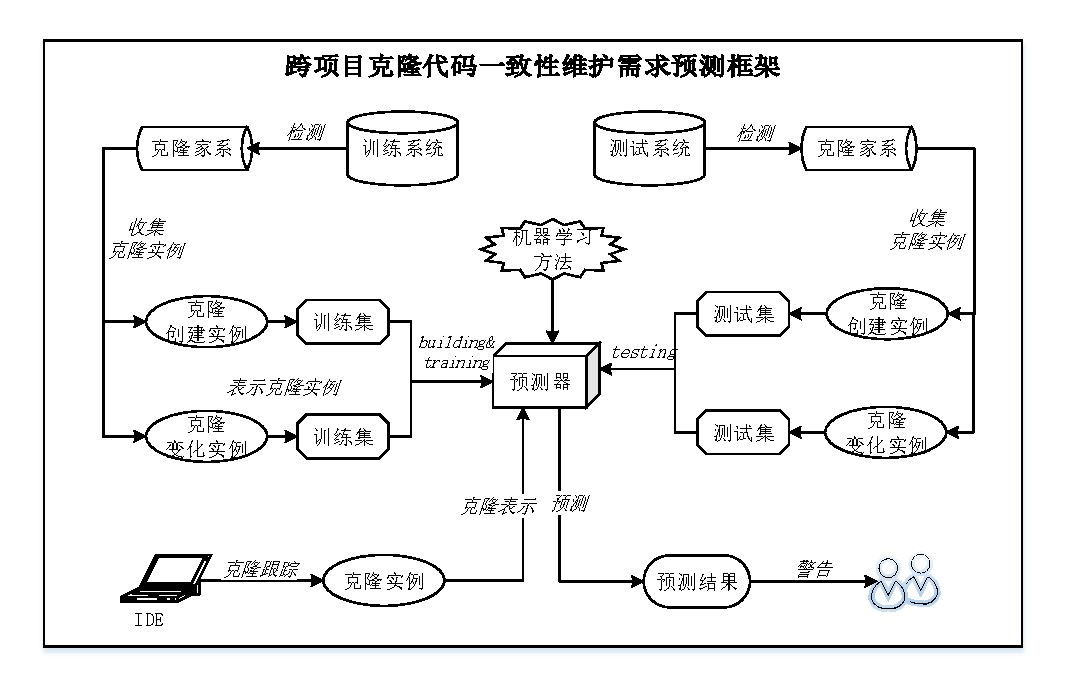
\includegraphics[width = 0.9\textwidth]{framework5.pdf}
\bicaption[framework5]{}{克隆代码一致性维护需求预测实证研究框架}
{Fig.$\!$}{The framework for empirical study on clone consistency-requirement prediction }
\vspace{-1em}
\end{figure}

一般来说,预测任务总是需要某些特征的知识,这些特征是我们工作中这些属性的编码向量。对于不同的克隆和变化的实例,预测属性是不可避免的,这些实例来自于他们的危险的工作\cite{wang2014predicting} \cite{zhang2016predicting}。
具体来说,使用代码属性和上下文属性来克隆克隆实例,并且采用新的进化属性,并结合来自克隆组视角的不同的代码和上下文属性来克隆变更实例。
%同样地,由Wang 构建的预测,我们从代码和上下文角度增加了两个变体属性集 - 借给他们预测克隆克隆实例,并从克隆谱系角度和可变性属性集中提取新的进化属性集从克隆变化的角度 - 借鉴它们来预测克隆变化实例。
此外,下一个预测的基本知识是采用不同机器学习方法的技术。
在我们的表现预测中,我们考虑五种不同的学习方法如下:\textcolor{red}{\em 贝叶斯网络分类器\cite{friedman1997bayesian},本机贝叶斯分类器\cite{john1995estimating},支持向量机分类器\cite{platt199912} K-Nearest Neighbors classifier \cite{aha1991instance}和决策树分类器\cite{quinlan2014c4}}。
我们执行和比较所有这五种机器学习方法,以帮助开发人员选择一种克隆和改变实际预测的一般技术。

\BiSection{克隆实例收集与表示}
{The Framework for Clone Consistency-Requirement base on Machine Learning}

\BiSubsection{克隆实例收集}
{Collecting Clone Instances}

收集克隆实例的目的是生成预测模型的训练数据。所有的克隆实例都可以从软件仓库的克隆系谱中获得。我们按照Kim et.al \cite {kim2005empirical}提出的方法构建软件的所有克隆系谱,我们还克隆了克隆组与1型和2型变化模式的克隆变化模式,应用于单独克隆克隆和更改实例。具体来说,为了从软件库中构建克隆系谱,我们首先使用NiCad \cite{roy2008nicad}从每个版本的软件仓库中检测出所有克隆片段和组。然后,我们将每个两个相邻软件版本之间的所有克隆组映射,以识别克隆组在这两个版本中的所有克隆进化关系。 并且还可以揭示克隆组的克隆变化模式。对于一对映射的克隆组,我们可以通过计算此映射中的克隆片段的类型1和2一致变化中来确定类型1和类型-2的克隆更改模式克隆组。然后,克隆组将被其拥有的变化模式标记(如定义}中所述)。具体来说,我们首先为每个克隆片段生成一个{\em 克隆区域描述符} $ \mathit {CRD} $,其细节在\cite{Duala2010}中描述。然后我们使用一个称为{\em CRD的克隆组映射算法}的映射算法来映射两个连续版本之间的所有克隆片段和克隆组。根据地图结果,我们为软件仓库构建了克隆谱系。此工作的详细信息可以在\cite{Ci2013}中找到。对于每个克隆组,我们确定其克隆模式。这需要检查此克隆组与其直接前身之间的一致变化(由克隆谱系提供)。一致变化的实际计算在定义\ref {defn-1}中指定。
接下来,克隆组将被它拥有的改变模式标记(如定义\ref {defn-2}中所述)。

可以通过遍历软件的所有克隆系谱来完成所有克隆克隆和更改实例的收集任务(定义\ref {defn-3})。对于克隆克隆实例,如果克隆组仅具有两个克隆片段,则可以通过检查是否可以将任何克隆片段映射到先前软件版本中的某些代码片段来确认被复制和粘贴的代码。如果有一个映射,则该克隆片段是复制的代码,另一个是粘贴的代码。如果没有人映射,随机的可以看起来是复制的代码。如果克隆组有多个克隆片段,我们似乎是这个克隆组,包括多个克隆克隆实例。\footnote{幸运的是,大多数克隆组只有两个片段,所以这个决定不会影响我们的克隆预测。}

\BiSubsection{克隆实例表示}
{Representing Clone Instances}

应用机器学习方法来预测克隆一致性,我们使用向量属性代替克隆实例,而不是直接使用代码片段或克隆组。因此,从克隆片段和克隆组中提取不同的属性集,以捕获克隆克隆实例和更改实例的相关信息。我们使用两个属性集的代码和上下文适应克隆克隆实例,这是由Wang等人预测的。 \cite{wang2014predicting}。
同时,我们选择了代码和上下文属性集以及克隆更改实例的进化属性集,这是Zhang等人预测的结果。 \cite{zhang2016predicting}。

具体来说,我们考虑克隆克隆实例中的复制和粘贴代码的不同属性集,其中为复制的代码属性和粘贴代码的上下文属性。
代码属性捕获克隆实例中复制的代码的特征,包括:{\em 代码行数,参数数,调用调用次数,包含halstead数,语法语句数。}
{\em numbers of lines of code, number of parameters, number of call invocations, number of include halstead, number of syntactic statement.}
更重要的是,上下文属性集包含克隆实例中复制的代码和粘贴代码之间的上下文信息,包括克隆的{\em locality,文件名相似性及其掩码,方法名称相似性,参数相似性和其类型的和 ,参数相似度的最大值及其类型,以及块信息。}{\em locality of clones, file name similarity and its' mask, method name similarity, sum of parameter similarity and its type, maximal of parameter similarity and its type, and block information.} \footnote{我们从Wang等人中删除了预测的历史属性集,这些属性被链接到复制代码的历史,而不是克隆实例。}

此外,三组属性是聚集器,用于捕获组中克隆更改实例的特性。前两个属性集与具有代码和上下文属性集的克隆实例类似,其中主要区别在于从克隆组角度来计算它们。
具体来说,代码属性和上下文属性与克隆实例的收集类似,主要区别在于我们计算克隆组中的值,而不仅仅是两个克隆。克隆更改实例的最终属性集是由系谱获得的
克隆组的特征,包括{\em 克隆组年龄,克隆模式数,模式当前,克隆更改摘要和更改信息。}
{\em clone group age, number of clone patterns, current of pattern, summaries of clone changes and change information.}



\BiSection{机器学习方法介绍}
{The Brief Introduction of Employed Machine Learning Methods}



\BiSection{训练和预测}
{predicting}

对于每个主题软件仓库,我们通过提取克隆克隆和更改实例的所有相应属性来构建两个不同的训练数据集。这个预测任务是一个监督的学习工作,所以最后的准备工作是将每个实例与一致性要求/一致性指示相关联 - 如定义\ref {defn-4}所定义。使用这些标记的数据集,我们可以用预测任务的一些特定的机器学习方法来构建我们的预测变量。在我们的工作中,我们的目标是通过更多的机器学习方法来预测这个问题,以探索我们的研究问题,因此在我们的实验中,我们将为克隆克隆和更改实例构建和训练机器学习方法的多个预测因子。

当克隆克隆和更改实例发生时,我们打算为开发人员提供克隆一致性要求的这些预测因子。如图所示,这些预测变量可以集成到一个IDE中,如eclipse,可以帮助开发人员在开发阶段维护克隆的克隆和变化。这需要追踪克隆克隆和更改的其他要求,这可以由IDE支持。已经超出了我们的研究范围。当开发人员克隆或更改克隆片段时,已使用提取的属性生成克隆克隆或更改实例,并引用此实例。相关预测器将预测其一致性要求,并根据需要通知开发人员采取措施维护此代码克隆。

\BiSection{插件实现}
{Implementation as a Plug-in}


\BiSection{实验结果与分析}
{Experiments Results and Analysis}

\begin{table*}[ht]
%%\caption{The four open source projects for experiments}
%%\label{allprojects}
\bicaption[allprojects]{}{不同机器学习方法的预测效果}
{Table$\!$}{The four open source projects for experiments}
\vspace{0.5em}
\centering
\wuhao
\begin{tabular}{ccccc}
\toprule[1.5pt]
~\multirow{2}{*}{\textbf{Instances}}&\multirow{2}{*}{\textbf{Project}}&\textbf{Consistency-} &\textbf{Meeting} &\multirow{2}{*}{\textbf{Total}}\\
~&~&\textbf{Requirement Free}&\textbf{Consistency-Requirement}&~\\
\midrule[1pt]
\multirow{4}{*}{\textbf{Cloning}}
&ArgoUML&	2574(77.07\%)&	766(22.93\%)&	3340\\
&jEdit&560(88.47\%)&	73(11.53\%)&	633\\
&jFreeChart&	2013(59.80\%)&	1353(40.20\%)&	3366\\
&Tuxguitar&	1016(71.10\%)&	413(28.90\%)&	1429\\
\hline
\multirow{4}{*}{\textbf{Changing}}
&ArgoUML&288(67.45\%)&139(32.55\%)&427\\
&jEdit&78(49.06\%)&81(50.94\%)&159\\
&jFreeChart&452(43.46\%)&588(56.54\%)&1040\\
&Tuxguitar&91(25.71\%)&263(74.29\%)&354\\
\bottomrule[1.5pt]
\end{tabular}
\end{table*}

%%\begin{table*}[ht]
%%%% increase table row spacing, adjust to taste
%%%\renewcommand{\arraystretch}{1.3}
%%% if using array.sty, it might be a good idea to tweak the value of
%%% \extrarowheight as needed to properly center the text within the cells
%%\caption{The four open source projects for experiments}
%%\label{projects}
%%\centering
%%%% Some packages, such as MDW tools, offer better commands for making tables
%%%% than the plain LaTeX2e tabular which is used here.
%%\begin{tabular}{|c|c|c|c|c|c|c|}
%%\hline
%%~\multirow{3}{*}{\textbf{Project}}& \multicolumn{3}{|c|}{\textbf{Number (Percentage) of Cloning Instances}} &  \multicolumn{3}{|c|}{\textbf{Number (Percentage) of Changing Instances}} \\ 
%% \cline{2-7}
%%~&\textbf{Consistency-} &\textbf{Meeting} &\multirow{2}{*}{\textbf{Total}}& \textbf{Consistency-} &\textbf{Meeting} &\multirow{2}{*}{\textbf{Total}}\\
%%~&\textbf{Requirement Free}&\textbf{Consistency-Requirement}&~&\textbf{Requirement Free}&\textbf{Consistency-Requirement}&\\
%%\hline
%%ArgoUML&	2574(77.07\%)&	766(22.93\%)&	3340&288(67.45\%)&139(32.55\%)&427\\
%%\hline
%%jEdit&560(88.47\%)&	73(11.53\%)&	633&78(49.06\%)&81(50.94\%)&159\\
%%\hline
%%jFreeChart&	2013(59.80\%)&	1353(40.20\%)&	3366&452(43.46\%)&588(56.54\%)&1040\\
%%\hline
%%Tuxguitar&	1016(71.10\%)&	413(28.90\%)&	1429&91(25.71\%)&263(74.29\%)&354\\
%%\hline
%MORE&	 &	 &	&&&\\\hline
%%\end{tabular}
%%\end{table*}

为了解决我们的研究问题,我们对{四}开源项目进行了实验。
表\ref{projects}显示了这些项目的细节,用于克隆克隆和更改状态。从该表可以看出,克隆克隆实例的数量范围为633到3666个,更改实例的范围为159到1040个,项目{\em jEdit}是最小的存储库。具体来说,列3和列6中列出了满足一致性要求的两个类型克隆实例(即,导致将来克隆组一致变化)的数量,而第2列和第5列反映了克隆实例的数量是一致性要求免费的(即,{\em not \/}将导致任何一致的变化)。

我们可以从Table\ref{projects}对克隆实例有两个观察结果。对于克隆克隆实例,{\em  三个项目}有数千个克隆克隆实例,而{\em jEdit}则有超过一千个。这些克隆实例中只有一小部分符合一致性要求,范围从12\%到40\%。这表明克隆操作已经成为开发人员的常用技术,并且大多数人不会在将来引入一致的变化,这意味着开发人员可以面对这种技术。另一方面,对于克隆更改实例,{\em  三}项目只有数百个变化的实例,而对于{\em  jFreeChart}则只有1040个计数,这意味着这些克隆中的大多数不会在演化中改变频率。尽管如此,满足一致性要求的变更实例占所有变更实例的33%至74%的百分比。换句话说,还有几百个改变实例的机会,导致将来一致的变化或克隆缺陷。因此,开发人员应该更加注意软件开发中的克隆变化。

在我们的实验中,我们的目标是解决三个子问题的研究问题,以便将这些实验分为三个部分。对于第一个研究问题,我们构建了克隆克隆实例的{\em 克隆克隆实验},显示了{\em 五种不同机器学习方法的有效性}。类似地,克隆更改实验是为克隆更改实例构建的。应该指出的是,这两个实验之间的讨论是针对第三个研究问题提供的,我们根据开发人员在实践中应用这些预测模型的调查提供了我们的建议。
与不同的是,根据我们预测任务的标签,我们克隆克隆和变更实例的实验可以自然地分为两部分:满足一致性要求和满足一致性。
这些满足一致性的情况将导致未来的一致变化,我们警告开发商应采取相应措施。
另一方面,满足一致性的这些实例不会,开发人员可以自由地自行复制或更改代码。

与\cite{wang2014predicting} \cite{zhang2016predicting}中执行的作品类似,我们从两个不同的角度评估我们的预测的有效性。首先,{\em  效果实验\/}:我们利用不同机器学习方法从四个项目中提取的所有属性来训练和测试模型,并评估预测的质量。
第二,{\em 属性集实验\/}:我们用不同的机器学习方法评估三个贡献属性集中的每一个对预测质量的影响。
\textcolor{red}{为了评估每个预测的有效性,我们采用了{\em Percision,Recall和F-Measure}的三个度量。}

在我们的案例研究中,采用五种机器学习方法来探索这四个项目的这些预测的有效性。我们没有意图改进这些方法来适应这种一致性要求的预测。
因此,我们使用包装WEKA来建立和训练我们所有需要的预测模型与不同的机器学习方法。WEKA是一种非常灵活且易于使用的数据挖掘工具,其中包含大量的分类/预测方法\cite{hall2009weka}。
在本节中,我们将使用每种机器学习方法的缩写术语,贝叶斯网络为{\em BayesNet},本机贝叶斯为{\em Native},支持向量机为{\em SVM},K最近邻居作为{\em KNN}和设计树作为{\em 树}详细。

\BiSubsection{平均}
{Experiments for Clone Consistency-Requirement}
在本实验中,我们解决了克隆克隆实例的第一个子研究问题。
{\em {子问题1:}
在克隆克隆时间,其他机器学习方法是否可以用于克隆一致性要求预测?
属性集是否对此预测产生积极或消极的影响?}
我们采用五种不同的机器学习方法来预测这四个项目的克隆一致性,因此预测结果如表。

\begin{table}[htbp]
%%\caption{The Average Effectiveness of Cloning Instances}
%%\label{cloningallavg}
\bicaption[cloningallavg]{}{不同机器学习方法的预测效果}
{Table$\!$}{The Average Effectiveness of Cloning Instances}
\vspace{0.5em}
\centering
\wuhao
\begin{tabular}{cccccc}
\toprule[1.5pt]
{\textbf{Metric}}&{\textbf{Method}}&{\textbf{ArgoUML}}&{\textbf{jEdit}}&{\textbf{jFreeChart}}&{\textbf{Tuxguitar}}\\
\midrule[1pt]
\multirow{5}{*}{Percision}
&{BayesNet}&0.935&0.889&0.883&	0.831\\
&{Native}&	0.886&	0.871&	0.869&	0.793\\
&{SVM}&0.958&	0.924&0.906&0.888\\
&{KNN}&	0.94&0.886&0.9&	0.848\\
&{Tree}	&0.939&0.898	&0.893&0.889\\
\hline
\multirow{5}{*}{Recall}
&{BayesNet}& 0.936&	0.877&	0.882&	0.836\\
&{Native}&0.888&0.82&	0.868&0.794\\
&{SVM}& 0.958&0.921&0.904&0.883\\
&{KNN}&0.94&0.889&	0.9	&0.848\\
&{Tree}&0.94	&0.905&	0.892&0.891\\
\hline
\multirow{5}{*}{F-Measure}
&{BayesNet}&0.935&0.882&0.881&0.832\\
&{Native}&0.887&	0.84&0.867&0.794\\
&{SVM}&0.957&	0.903	&0.903&0.876\\
&{KNN}&0.94&0.887&	0.9	&	0.848\\
&{Tree}	&0.939&	0.901	&0.892&0.89\\
\bottomrule[1.5pt]
\end{tabular}
\end{table}

\begin{table}[htbp]
%%\caption{The Effectiveness of Cloning Instances for free}
%%\label{cloningallfree}
%%\center
\bicaption[cloningallfree]{}{克隆创建实例的一致性自由的预测效果}
{Table$\!$}{The Effectiveness of Cloning Instances for Consistency-Free}
\vspace{0.5em}
\centering
\wuhao
\begin{tabular}{cccccc}
\toprule[1.5pt]
{\textbf{Metric}}&{\textbf{Method}}&{\textbf{ArgoUML}}&{\textbf{jEdit}}&{\textbf{jFreeChart}}&{\textbf{Tuxguitar}}\\
\midrule[1pt]
\multirow{5}{*}{Percision}
&{BayesNet	}&0.945	&0.943	&0.879	&0.861\\
&{Natvie	}&0.917	&0.941	&0.863	&0.853\\
&{SVM}&	0.955	&0.919	&0.889	&0.872\\
&{KNN}&	0.96	&0.933	&0.905&	0.891\\
&{J48}&	0.953&	0.936	&0.891	&0.913\\
\hline
\multirow{5}{*}{Recall}
&{BayesNet}&	0.974&	0.916&	0.932	&0.917\\
&{Natvie	}&0.94&	0.85&	0.927	&0.858\\
&{SVM}&	0.992	&0.998	&0.959&	0.979\\
&{KNN}&	0.962&	0.943	&0.93	&0.896\\
&{J48}&	0.969&	0.959&	0.934&	0.935\\
\hline
\multirow{5}{*}{F-Measure}
&{BayesNet}&	0.959	&0.929&	0.905&	0.888\\
&{Natvie	}&0.928	&0.893	&0.894	&0.856\\
&{SVM}&	0.973	&0.957&	0.923	&0.923\\
&{KNN}&	0.961&	0.938	&0.917	&0.893\\
&{J48}&     0.961&	0.947	&0.912&	0.924\\
\bottomrule[1.5pt]
\end{tabular}
\end{table}

\begin{table}[htbp]
%%\caption{The Effectiveness of Cloning Instances for Meeting Consistency-Requirement}
%%\label{cloningallmeeting}
\bicaption[cloningallmeeting]{}{符合研究生院绘图规范的表格}{Table$\!$}
{The Effectiveness of Cloning Instances for  Meeting Consistency-Requirement}
\vspace{0.5em}
\wuhao
\centering
\begin{tabular}{cccccc}
\toprule[1.5pt]
{\textbf{Metric}}&{\textbf{Method}}&{\textbf{ArgoUML}}&{\textbf{jEdit}}&{\textbf{jFreeChart}}&{\textbf{Tuxguitar}}\\
\midrule[1pt]
\multirow{5}{*}{Percision}
&{BayesNet}&	0.808	&0.575	&0.809	&0.637\\
&{Natvie}&	0.714	&0.589	&0.78	&0.637\\
&{SVM}&	0.845	&0.329	&0.823	&0.646\\
&{KNN}&	0.864	&0.479	&0.854	&0.731\\
&{J48}&	0.841	&0.493	&0.831	&0.782\\
\hline
\multirow{5}{*}{Recall}
&{BayesNet}&	0.902	&0.472	&0.889	&0.758\\
&{Natvie}&	0.78	&0.339	&0.878	&0.646\\
&{SVM}&	0.969	&0.96	&0.931	&0.927\\
&{KNN}&	0.872	&0.522	&0.892	&0.74\\
&{J48}&	0.891	&0.61	&0.894	&0.83\\
\hline
\multirow{5}{*}{F-Measure}
&{BayesNet}&	0.853	&0.519	&0.847	&0.692\\
&{Natvie}&	0.746	&0.43	&0.826	&0.641\\
&{SVM}&	0.902	&0.49	&0.873	&0.762\\
&{KNN}&	0.902	&0.49	&0.873	&0.762\\
&{J48}&	0.865	&0.545	&0.861	&0.805\\
\bottomrule[1.5pt]
\end{tabular}
\end{table}




\begin{table*}[htbp]
%%\caption{The Average Effectiveness of Attribute Set for Cloning Instances}
%%\label{cloningsetavg}
\bicaption[cloningsetavg]{}{符合研究生院绘图规范的表格}{Table$\!$}
{The Average Effectiveness of Attribute Set for Cloning Instances}
\vspace{0.5em}
\centering
\scriptsize
\begin{tabular}{cccccccccccccc}
\toprule[1.5pt]
\multirow{2}{*}{\textbf{Metric}}&\multirow{2}{*}{\textbf{Method}}&\multicolumn{3}{c}{\textbf{ArgoUML}}&\multicolumn{3}{c}{\textbf{jEdit}}&\multicolumn{3}{c}{\textbf{jFreeChart}}&\multicolumn{3}{c}{\textbf{Tuxguitar}}\\
\cline{3-14}
&&\textbf{All}&\textbf{Code}&\textbf{Context}&\textbf{All}&\textbf{Code}&\textbf{Context}&\textbf{All}&\textbf{Code}&\textbf{Context}&\textbf{All}&\textbf{Code}&\textbf{Context}~\\
\midrule[1pt]
\multirow{5}{*}{Percision}
&BayesNet&	0.935&	0.912&	0.917&		0.889&	0.885&	0.83&		0.883&	0.808&	0.903&		0.831&	0.811&	0.843\\
&Native&	0.886&	0.866&	0.877&		0.871&	0.865&	0.832&		0.869&	0.755&	0.873&		0.793&	0.747&	0.824\\
&SVM&	0.958&	0.928&	0.942&		0.924&	0.924&	0.909&		0.906&	0.819&	0.906&		0.888&	0.834&	0.873\\
&KNN&	0.94&	0.911&	0.933&		0.886&	0.903&	0.877&		0.9	&0.808&	0.898&		0.848&	0.806&	0.861\\
&Tree&	0.939&	0.904&	0.93&		0.898&	0.882&	0.876&		0.893&	0.802&	0.891&		0.889&	0.8&	0.881\\
\hline
\multirow{5}{*}{Recall}
&BayesNet&	0.936&	0.914&	0.919&		0.877&	0.869&	0.852&		0.882&	0.803&	0.903&		0.836&	0.817&	0.846\\
&Native&	0.888&	0.868&	0.88&		0.82&	0.836&	0.826&		0.868&	0.752&	0.873&		0.794&	0.756&	0.816\\
&SVM&	0.958&	0.929&	0.943&		0.921&	0.921&	0.918&		0.904&	0.806&	0.904&		0.883&	0.837&	0.874\\
&KNN&	0.94&	0.912&	0.934&		0.889&	0.912&	0.885&		0.9&	0.803&	0.898&		0.848&	0.81&	0.862\\
&Tree&	0.94&	0.905&	0.931&		0.905&	0.896&	0.889&		0.892&	0.796&	0.89&		0.891&	0.807&	0.882\\
\hline
\multirow{5}{*}{F-Measure}
&BayesNet&	0.935&	0.912&	0.917&		0.882&	0.876&	0.84&		0.881&	0.797&	0.902&		0.832&	0.811&	0.844\\
&Native&	0.887&	0.867&	0.878&		0.84&	0.848&	0.829&		0.867&	0.741&	0.872&		0.794&	0.75&	0.819\\
&SVM&	0.957&	0.927&	0.941&		0.903&	0.903&	0.907&		0.903&	0.797&	0.903&		0.876&	0.827&	0.869\\
&KNN&	0.94&	0.912&	0.933&		0.887&	0.905&	0.881&		0.9&	0.796&	0.897&		0.848&	0.807&	0.862\\
&Tree&	0.939&	0.904&	0.93&		0.901&	0.887&	0.881&		0.892&	0.788&	0.889&		0.89&	0.802&	0.881\\
\bottomrule[1.5pt]
\end{tabular}
\end{table*}


\begin{table*}[htbp]
\scriptsize
%%\caption{The Effectiveness of Attribute Set for Cloning Instances for free}
%%\label{cloningsetfree}
\bicaption[cloningsetfree]{}{符合研究生院绘图规范的表格}{Table$\!$}
{The Effectiveness of Attribute Set for Cloning Instances for Consistency-Requirement Free}
\vspace{0.5em}
\centering
\begin{tabular}{cccccccccccccc}
\toprule[1.5pt]
\multirow{2}{*}{\textbf{Metric}}&\multirow{2}{*}{\textbf{Method}}&\multicolumn{3}{c}{\textbf{ArgoUML}}&\multicolumn{3}{c}{\textbf{jEdit}}&\multicolumn{3}{c}{\textbf{jFreeChart}}&\multicolumn{3}{c}{\textbf{Tuxguitar}}\\
\cline{3-14}
&&\textbf{All}&\textbf{Code}&\textbf{Context}&\textbf{All}&\textbf{Code}&\textbf{Context}&\textbf{All}&\textbf{Code}&\textbf{Context}&\textbf{All}&\textbf{Code}&\textbf{Context}~\\
\midrule[1pt]
\multirow{5}{*}{Percision}
&BayesNet&0.945&	0.932	&0.929&		0.943&	0.942	&0.9	&	&0.879	&0.789	&0.898		&0.861	&0.848	0.88\\
&Native&0.917	&0.907&	0.913	&	0.941	&0.932&	0.906	&	0.863&	0.744&	0.873	&	0.853&	0.809	&0.89\\
&SVM&0.955&	0.937	&0.945	&	0.919	&0.919&	0.928&		0.889	&0.779&	0.889	&	0.872	&0.843	&0.877\\
&KNN&0.96	&0.94	&0.947	&	0.933&	0.934	&0.926	&	0.905&	0.787&	0.896	&	0.891&	0.856&	0.9\\
&Tree&0.953&	0.936	&0.943	&	0.936&	0.923	&0.921&		0.891&	0.778&	0.884	&	0.913	&0.842&	0.907\\

\hline
\multirow{5}{*}{Recall}
&BayesNet&0.974	&0.958	&0.969	&	0.916	&0.907&	0.936		&0.932	&0.916	&0.944	&	0.917	&0.905	&0.906\\
&Native&0.94	&0.924	&0.933&		0.85	&0.879&	0.896		&0.927&	0.892	&0.922	&	0.858	&0.86&	0.845\\
&SVM&0.992	&0.973&	0.983		&0.998	&0.998&	0.984		&0.959	&0.944	&0.959		&0.979	&0.947	&0.957\\
&KNN&0.962&	0.946&	0.969	&	0.943	&0.968&	0.945		&0.93&	0.919&	0.937	&	0.896	&0.881&	0.907\\
&Tree&0.969&	0.941	&0.969	&	0.959&	0.963	&0.957	&	0.934	&0.92&	0.939	&	0.935	&0.897	&0.93\\
\hline
\multirow{5}{*}{F-Measure}
&BayesNet&0.959&	0.945&	0.949	&	0.929	&0.924&	0.918	&	0.905&	0.848	&0.921	&	0.888&	0.875&	0.893\\
&Native&0.928&	0.915	&0.923	&0.893	&0.904	&0.901		&0.894&	0.811&	0.897	&	0.856	&0.834	&0.867\\
&SVM&0.973&	0.955&	0.964	&	0.957&	0.957&	0.955	&	0.923&	0.854	&0.923&		0.923&	0.892&	0.915\\
&KNN&0.961&	0.943&	0.958	&	0.938	&0.951&	0.935		&0.917	&0.848	&0.916&		0.893&	0.868	&0.903\\
&Tree&0.961&	0.938&	0.956	&	0.947	&0.942&	0.939	&	0.912&	0.843	&0.911&		0.924	&0.868&	0.918\\
\bottomrule[1.5pt]
\end{tabular}
\end{table*}


\begin{table*}[htbp]
\scriptsize
%%\caption{The Effectiveness of Attribute Set for Cloning Instances for meeting}
%%\label{cloningsetmeeting}
\bicaption[sdfj1]{}{符合研究生院绘图规范的表格}{Table$\!$}
{The Effectiveness of Attribute Set for Cloning Instances for Meeting Consistency-Requirement}
\vspace{0.5em}
\centering
\begin{tabular}{cccccccccccccc}
\toprule[1.5pt]
\multirow{2}{*}{\textbf{Metric}}&\multirow{2}{*}{\textbf{Method}}&\multicolumn{3}{c}{\textbf{ArgoUML}}&\multicolumn{3}{c}{\textbf{jEdit}}&\multicolumn{3}{c}{\textbf{jFreeChart}}&\multicolumn{3}{c}{\textbf{Tuxguitar}}\\
\cline{3-14}
&&\textbf{All}&\textbf{Code}&\textbf{Context}&\textbf{All}&\textbf{Code}&\textbf{Context}&\textbf{All}&\textbf{Code}&\textbf{Context}&\textbf{All}&\textbf{Code}&\textbf{Context}~\\
\midrule[1pt]
\multirow{5}{*}{Precision}
&BayesNet&	0.902	&0.844	&0.878	&	0.472	&0.447	&0.294	&	0.889	&0.836	&0.91	&	0.758	&0.719	&0.752\\
&Native&	0.78&	0.728&	0.756	&	0.339	&0.352	&0.266	&	0.878	&0.772	&0.873	&	0.646	&0.593	&0.662\\
&SVM&	0.969	&0.896	&0.934	&	0.96	&0.96&	0.769	&	0.931	&0.879	&0.931	&	0.927&	0.813	&0.863\\
&KNN&	0.872	&0.815	&0.888		&0.522	&0.66	&0.5		&0.892	&0.839	&0.9	&	0.74&	0.684	&0.767\\
&Tree&	0.891	&0.799&	0.885	&	0.61	&0.571	&0.529	&	0.894	&0.837&	0.901	&	0.83	&0.697	&0.817\\
\hline
\multirow{5}{*}{Recall}
&BayesNet&	0.808	&0.765&	0.752		&0.575	&0.575	&0.205	&	0.809&	0.636&	0.841	&	0.637&	0.6	&0.697\\
&Native&	0.714&	0.68	&0.701	&	0.589	&0.507&	0.288		&0.78	&0.542	&0.8	&	0.637	&0.501	&0.743\\
&SVM&	0.845&	0.779	&0.808	&	0.329	&0.329&	0.411	&	0.823	&0.601&	0.821	&	0.646	&0.567	&0.671\\
&KNN&	0.864&	0.798	&0.816	&	0.479	&0.479&	0.425	&	0.854&	0.63&	0.838		&0.731	&0.634&	0.751\\
&Tree&	0.841&	0.782	&0.803	&	0.493	&0.384&	0.37	&	0.831&	0.61&	0.817	&	0.782	&0.586	&0.765\\
\hline
\multirow{5}{*}{F-Measure}
&BayesNet&	0.853&	0.803&	0.81	&	0.519	&0.503&	0.242	&	0.847&	0.722&	0.874	&	0.692&	0.654&	0.724\\
&Native&	0.746&	0.703	&0.728		&0.43	&0.416	&0.276	&	0.826	&0.637	&0.835		&0.641	&0.543	&0.7\\
&SVM&	0.902&	0.834&	0.866&		0.49&	0.49	&0.536	&	0.873&	0.714	&0.873	&	0.762	&0.668&	0.755\\
&KNN&	0.868&	0.806&	0.85	&	0.5&	0.556	&0.459		&0.873	&0.72	&0.868		&0.736&	0.658	&0.759\\
&Tree&	0.865&	0.79&	0.842	&	0.545&	0.459&	0.435	&	0.861	&0.706&	0.857	&	0.805	&0.637&	0.79\\
\bottomrule[1.5pt]
\end{tabular}
\end{table*}

表{克拉克隆}表示克隆实例预测的有效性。从这个表可以看出,这种方法可以通过五种不同的机器学习方法{\ em有效地预测克隆一致性要求,从79.3\%到95.8\%的准确度从79.4\%回归到95.8\% ,F值从79.4\%至95.7\%。
比较所采用的学习方法的有效性,显然,{\em SVM}具有比这四个项目的其他方法更好的克隆预测能力。具体来说,SVM对于{\em ArgoUML,jEdit和jFreeChart}具有最好的结果,决策树具有最好的结果,SVM对于{\em Tuxguitar}来说是第二好的。与此同时,贝叶斯网络和本地贝叶斯方法在这四个项目中几乎保持了相对较差的预测结果。
因此,我们建议开发人员在需要预测克隆实例时首先考虑SVM。

为了探索属性集如何影响预测效果,我们仅使用一个属性集进行预测。属性集有效性的结果如表\ref{cloningset}所示。在这个表中,我们为所有属性集使用“全部”列,分别为其属性集使用“代码”,“上下文”。从这个表中可以看出,在不同属性的三个预测中,并没有显着差异。这表明我们的属性集不会对我们的预测产生负面影响。然而,对于这三个预测,我们还可以看到,在所有这四个项目的“属性”预测列(仅代码或上下文)中存在大部分相对较差的预测。具体来说,这三个项目的“代码”列{\em ArgoUML \/},{\em jFreeChart \/}和{\em Tuxguitar}对于这五个方法都有最差的结果,而“上下文” “{\em jEdit}”项目的列对于这五种方法几乎都是最差的.此外,我们将这些预测的结果与五种机器学习方法进行比较,我们得出的结论与SVM具有较好的预测能力相同。因此,建议在该预测中保留所有属性集,并首先优选SVM方法。


根据表\ref{克拉克隆}和表\ref{cloningset},我们可以给出我们对子问题1的建议。在克隆时间,五种机器学习方法可以应用于这种克隆预测,其结果非常相似。另外,他们之间还是有一点区别,SVM有更好的能力,我们建议开发选择这个来预测。同时,我们的属性集实验表明,所选择的属性对这一预测具有积极的影响,我们建议开发者可以自信选择它们进行预测。

\BiSubsection{2}
{2}
在本节中,我们解决克隆更改实例的第二个问题。{\em
{子问题2:}
在克隆更改时间,其他机器学习方法是否可以用于克隆一致性要求预测?
属性集是否对我们的预测产生积极或消极的影响?
}
为了解决这个问题,我们采用了五种不同的机器学习方法进行克隆更改的一致性,结果如表。
\begin{table}[htbp]
%%\caption{The Average Effectiveness of Changing Instances}
%%\label{changingallavg}
\bicaption[changingallavg]{}{符合研究生院绘图规范的表格}
{Table$\!$}{The Average Effectiveness of Changing Instances}
\centering
\wuhao
\begin{tabular}{cccccc}
\toprule[1.5pt]
{\textbf{Project}}&{\textbf{Metric}}&{\textbf{ArgoUML}}&{\textbf{jEdit}}&{\textbf{jFreeChart}}&{\textbf{Tuxguitar}}\\
\midrule[1pt]
\multirow{5}{*}{Percision}
&{BayesNet}&0.724&	0.686&	0.791&0.72\\
&{Native}& 0.734&	0.696	&0.778&	0.729\\
&{SVM}&0.744	&0.704&0.793	&0.733\\
&{KNN}&0.733	&0.597&	0.772&	0.672\\
&{Tree}&0.682	&0.581	&0.742	&0.637\\
\hline
\multirow{5}{*}{Recall}
&{BayesNet}&0.735	&	0.686&0.791&0.746\\
&{Native}&0.726&	0.692&0.778&0.737\\
&{SVM}&0.752	&0.704&0.791&0.734\\
&{KNN}&0.731	&	0.597	&	0.77	&	0.706\\
&{Tree}&0.698&	0.579	&	0.742&0.672\\
\hline
\multirow{5}{*}{F-Measure}
&{BayesNet}&	0.726	&	0.686	&0.79	&0.726\\
&{Native}&0.729&	0.689&0.778&0.733\\
&{SVM}&0.729&0.704	&0.789&	0.733\\
&{KNN}&0.732	&0.597	&0.771	&	0.683\\
&{Tree}&0.632	&	0.573&	0.739&0.651\\
\bottomrule[1.5pt]
\end{tabular}
\end{table}


\begin{table}[htbp]
%%\scriptsize
%%\caption{The Effectiveness of Changing Instances for Consistency-Requirement Free}
%%\label{changingallfree}
\bicaption[changingallfree]{}{符合研究生院绘图规范的表格}
{Table$\!$}{The Effectiveness of Changing Instances for Consistency-Requirement Free}
\vspace{0.5em}
\centering
\wuhao
\begin{tabular}{cccccc}
\toprule[1.5pt]
{\textbf{Project}}&{\textbf{Metric}}&{\textbf{ArgoUML}}&{\textbf{jEdit}}&{\textbf{jFreeChart}}&{\textbf{Tuxguitar}}\\
\midrule[1pt]
\multirow{5}{*}{Precision}
&{BayesNet}&0.774	&0.679	&0.783	&0.508\\
&{Native}&0.813	&0.723	&0.743	&0.488\\
&{SVM}&0.761	&0.707&	0.804&	0.483\\
&{KNN}&0.806&	0.592	&0.726&	0.39\\
&{Tree}&0.703	&0.59	&0.742&	0.302\\
\hline
\multirow{5}{*}{Recall}			
&{BayesNet}&0.858	&0.679&	0.719&	0.33\\
&{Native}&0.771	&0.603	&0.748	&0.44\\
&{SVM}&0.92&	0.679&	0.688	&0.473\\
&{KNN}&0.792&	0.577	&0.757	&0.253\\
&{Tree}&0.955&	0.462	&0.624	&0.209\\
\hline
\multirow{5}{*}{F-Measure}
&{BayesNet}&0.814	&0.679	&0.75	&0.4\\
&{Native}&0.791	&0.657&	0.745&	0.462\\
&{SVM}&0.833	&0.693	&0.741	&0.478\\
&{KNN}&0.799&	0.584	&0.741	&0.307\\
&{Tree}&0.81	&0.518	&0.678&	0.247\\
\bottomrule[1.5pt]
\end{tabular}
\end{table}

\begin{table}[htbp]
%%\scriptsize
%%\caption{The Effectiveness of Changing Instances for meeting}
%%\label{changingallmeeting}
\bicaption[changingallmeeting]{}{符合研究生院绘图规范的表格}
{Table$\!$}{The Effectiveness of Changing Instances for Meeting Consistency-Requirement }
\vspace{0.5em}
\centering
\wuhao
\begin{tabular}{cccccc}
\toprule[1.5pt]
{\textbf{Project}}&{\textbf{Metric}}&{\textbf{ArgoUML}}&{\textbf{jEdit}}&{\textbf{jFreeChart}}&{\textbf{Tuxguitar}}\\
\midrule[1pt]
\multirow{5}{*}{Precision}
&{BayesNet}&0.62	&0.691&	0.797	&0.793\\
&{Native}&0.571	&0.67	&0.805	&0.813\\
&{SVM}&0.709&	0.702	&0.784	&0.819\\
&{KNN}&0.583	&0.602	&0.807	&0.769\\
&{Tree}&0.639&	0.571&	0.742&	0.753\\
\hline
\multirow{5}{*}{Recall}
&{BayesNet}&0.482&	0.691&	0.847&	0.89\\
&{Native}&0.633&	0.778&	0.801&	0.84\\
&{SVM}&0.403&	0.728&	0.871&	0.825\\
&{KNN}&0.604&	0.617	&0.781&	0.863\\
&{Tree}&0.165	&0.691&	0.833&	0.833\\
\hline
\multirow{5}{*}{F-Measure}
&{BayesNet}&0.543	&0.691	&0.821	&0.839\\
&{Native}&0.601&	0.72&	0.803	&0.826\\
&{SVM}&0.514&	0.715	&0.825&	0.822\\
&{KNN}&0.594	&0.61	&0.793	&0.814\\
&{Tree}&0.263&	0.626&	0.785&	0.791\\
\bottomrule[1.5pt]
\end{tabular}
\end{table}



\begin{table*}[htbp]
\scriptsize
%%\caption{The Average Effectiveness of Attribute Set for Changing Instances}
%%\label{changingsetavg}
\bicaption[changingsetavg]{}{符合研究生院绘图规范的表格}
{Table$\!$}{The Average Effectiveness of Attribute Set for Changing Instances}
\vspace{0.5em}
\centering
\begin{tabular}{cccccccccccccccccc}
\toprule[1.5pt]
\multirow{2}{*}{\textbf{Metric}}&\multirow{2}{*}{\textbf{Method}}&\multicolumn{4}{c}{\textbf{ArgoUML}}&\multicolumn{4}{c}{\textbf{jEdit}}&\multicolumn{4}{c}{\textbf{jFreeChart}}&\multicolumn{4}{c}{\textbf{Tuxguitar}}\\
\cline{3-18}
%%&&\textbf{All}&\textbf{Code}&\textbf{Context}&\textbf{Evolution}&\textbf{All}&\textbf{Code}&\textbf{Context}&\textbf{Evolution}&\textbf{All}&\textbf{Code}&\textbf{Context}&\textbf{Evolution}&\textbf{All}&\textbf{Code}&\textbf{Context}&\textbf{Evolution}~\\
&&\textbf{All}&\textbf{Code}&\textbf{Cont}&\textbf{Evo}&\textbf{All}&\textbf{Code}&\textbf{Cont}&\textbf{Evo}&\textbf{All}&\textbf{Code}&\textbf{Cont}&\textbf{Evo}&\textbf{All}&\textbf{Code}&\textbf{Con}&\textbf{Evo}~\\
\midrule[1pt]
\multirow{5}{*}{Percision}
&BayesNet&	0.724&	0.737&	0.712&	0.727&		0.686&	0.698&	0.673&	0.654&	0.791&	0.76&	0.773&	0.76&		0.72&	0.686&	0.672&	0.727\\
&Native&	0.734&	0.743&	0.693&	0.723&		0.696&	0.662&	0.636&	0.676&	0.778&	0.756&	0.731&	0.747&		0.729&	0.7	&0.69&	0.719\\
&SVM&	0.744&	0.737&	0.736&	0.758&		0.704&	0.749&	0.687&	0.642&		0.793&	0.742&	0.769&	0.775&		0.733&	0.678&	0.726&	0.699\\
&KNN&	0.733&	0.692&	0.688&	0.725&		0.597&	0.522&	0.617&	0.68&		0.772&	0.703&	0.744&	0.741&		0.672&	0.639&	0.659&	0.669\\
&Tree&	0.682&	0.689&	0.713&	0.696&		0.581&	0.579&	0.571&	0.595&		0.742&	0.746&	0.711&	0.733&		0.637&	0.621&	0.658&	0.634\\
\hline
\multirow{5}{*}{Recall}
&BayesNet&	0.735&	0.742&	0.724&	0.733&		0.686&	0.698&	0.673&	0.654&	0.791&	0.761&	0.774&	0.761&		0.746&	0.718&	0.709&	0.743\\
&Native&	0.726&	0.738&	0.681&	0.71&		0.692&	0.66&	0.635&	0.673&		0.778&	0.757&	0.732&	0.742&		0.737&	0.703&	0.686&	0.737\\
&SVM&	0.752&	0.742&	0.74&	0.766&		0.704&	0.748&	0.686&	0.642&		0.791&	0.739&	0.768&	0.775&		0.734&	0.678&	0.718&	0.698\\
&KNN&	0.731&	0.698&	0.689&	0.733&		0.597&	0.522&	0.616&	0.679&		0.77&	0.7	&0.742&	0.738&		0.706&	0.681&	0.689&	0.689\\
&Tree&	0.698&	0.7	&0.726&	0.703&		0.579&	0.579&	0.553&	0.591&		0.742&	0.745&	0.711&	0.734&		0.672&	0.653&	0.672&	0.678\\
\hline
\multirow{5}{*}{F-Measure}
&BayesNet&	0.726&	0.739&	0.715&	0.729&		0.686&	0.698&	0.673&	0.654&		0.79&	0.76&	0.772&	0.76&		0.726&	0.695&	0.683&	0.732\\
&Native&	0.729&	0.74&	0.686&	0.714&		0.689&	0.659&	0.634&	0.671&		0.778&	0.756&	0.731&	0.743&		0.733&	0.702&	0.688&	0.725\\
&SVM&	0.729&	0.712&	0.707&	0.75&	0.704&	0.748&	0.684&	0.642&		0.789&	0.733	&0.765&	0.773&		0.733&	0.678&	0.721&	0.698\\
&KNN&	0.732&	0.694&	0.688&	0.727&		0.597&	0.522&	0.616&	0.678&		0.771&	0.701&	0.743&	0.739&		0.683&	0.655&	0.671&	0.677\\
&Tree&	0.632&	0.634&	0.694&	0.635&		0.573&	0.577&	0.533&	0.584&		0.739&	0.741&	0.711&	0.731&		0.651&	0.635&	0.664&	0.651\\
\bottomrule[1.5pt]
\end{tabular}
\end{table*}

\begin{table*}[htbp]
\scriptsize
%%\caption{The Effectiveness of Attribute Set for Changing Instances for free}
%%\label{changingsetfree}
\bicaption[changingsetfree]{}{符合研究生院绘图规范的表格}
{Table$\!$}{The Effectiveness of Attribute Set for Changing Instances for Consistency-Requirement Free}
\vspace{0.5em}
\centering
\begin{tabular}{cccccccccccccccccc}
\toprule[1.5pt]
\multirow{2}{*}{\textbf{Metric}}&\multirow{2}{*}{\textbf{Method}}&\multicolumn{4}{c}{\textbf{ArgoUML}}&\multicolumn{4}{c}{\textbf{jEdit}}&\multicolumn{4}{c}{\textbf{jFreeChart}}&\multicolumn{4}{c}{\textbf{Tuxguitar}}\\
\cline{3-18}
%%&&\textbf{All}&\textbf{Code}&\textbf{Context}&\textbf{Evolution}&\textbf{All}&\textbf{Code}&\textbf{Context}&\textbf{Evolution}&\textbf{All}&\textbf{Code}&\textbf{Context}&\textbf{Evolution}&\textbf{All}&\textbf{Code}&\textbf{Context}&\textbf{Evolution}~\\
&&\textbf{All}&\textbf{Code}&\textbf{Cont}&\textbf{Evo}&\textbf{All}&\textbf{Code}&\textbf{Cont}&\textbf{Evo}&\textbf{All}&\textbf{Code}&\textbf{Cont}&\textbf{Evo}&\textbf{All}&\textbf{Code}&\textbf{Con}&\textbf{Evo}~\\
\midrule[1pt]
\multirow{5}{*}{Precision}
&BayesNet&0.774&	0.795	&0.769	&0.788		&0.679	&0.703	&0.667	&0.653		&0.783	&0.731	&0.764	&0.739	&	0.508	&0.424	&0.393	&0.5\\
&Native&0.813	&0.817	&0.781&	0.808	&	0.723	&0.676	&0.643	&0.697	&	0.743	&0.726&	0.698&	0.685	&	0.488	&0.42	&0.394	&0.486\\
&SVM&	0.761	&0.747	&0.744	&0.78	&	0.707	&0.732	&0.7	&0.633		&0.804	&0.759	&0.775	&0.77	&	0.483&	0.374	&0.455	&0.413\\
&KNN&	0.806	&0.766	&0.768	&0.782	&	0.592	&0.513	&0.602	&0.69		&0.726	&0.644	&0.697	&0.688		&0.39	&0.31	&0.354	&0.37\\
&Tree&	0.703&	0.704	&0.738	&0.705	&	0.59	&0.58&	0.531	&0.61		&0.742	&0.749	&0.666	&0.724		&0.302	&0.265	&0.342	&0.298\\
\hline
\multirow{5}{*}{Recall}
&BayesNet&0.858&	0.833	&0.844	&0.826	&	0.679&	0.667	&0.667	&0.628	&	0.719	&0.71	&0.695	&0.695&		0.33	&0.275	&0.242&	0.396\\
&Native&0.771	&0.788	&0.733	&0.747	&	0.603&	0.59&	0.577	&0.59	&	0.748	&0.708	&0.675	&0.752	&	0.44	&0.407	&0.407&	0.374\\
&SVM&	0.92	&0.934&	0.938&	0.91	&	0.679	&0.769	&0.628	&0.641&		0.688&	0.586	&0.657	&0.688	&	0.473	&0.374	&0.495	&0.418\\
&KNN&	0.792	&0.795	&0.771	&0.837		&0.577	&0.526	&0.641	&0.628		&0.757	&0.692	&0.721	&0.73	&	0.253	&0.198	&0.253	&0.297\\
&Tree&	0.955	&0.958	&0.92&	0.962		&0.462	&0.513	&0.769&	0.462&		0.624&	0.622&	0.67&	0.626&		0.209&	0.198&	0.297&	0.187\\
\hline
\multirow{5}{*}{F-Measure}
&BayesNet&0.814&	0.814	&0.805&	0.807	&	0.679&	0.684	&0.667	&0.641	&	0.75	&0.721&	0.728	&0.716	&	0.4	&0.333&	0.299	&0.442\\
&Native&0.791&	0.802&	0.756&	0.776		&0.657	&0.63&	0.608	&0.639	&	0.745	&0.717	&0.686	&0.717	&	0.462&	0.413	&0.4	&0.422\\
&SVM&	0.833	&0.83&	0.829&	0.84&		0.693&	0.75&	0.662&	0.637&		0.741&	0.662&	0.711&	0.727&		0.478&	0.374&	0.474	&0.415\\
&KNN&	0.799	&0.78	&0.769&	0.809&		0.584	&0.519	&0.621	&0.658	&	0.741	&0.667	&0.709	&0.708	&	0.307	&0.242	&0.295	&0.329\\
&Tree&	0.81	&0.812	&0.819&	0.814&		0.518&	0.544&	0.628&	0.526&		0.678&	0.68&	0.668	&0.671&		0.247&	0.226&	0.318&	0.23\\
\bottomrule[1.5pt]
\end{tabular}
\end{table*}

\begin{table*}[htbp]
\scriptsize
%%\caption{The Effectiveness of Attribute Set for Changing Instances for meeting}
%%\label{changingsetmeeting}
\bicaption[changingsetmeeting]{}{符合研究生院绘图规范的表格}
{Table$\!$}{The Effectiveness of Attribute Set for Changing Instances for Meeting Consistency-Requirement}
\vspace{0.5em}
\centering
\begin{tabular}{cccccccccccccccccc}
\toprule[1.5pt]
\multirow{2}{*}{\textbf{Metric}}&\multirow{2}{*}{\textbf{Method}}&\multicolumn{4}{c}{\textbf{ArgoUML}}&\multicolumn{4}{c}{\textbf{jEdit}}&\multicolumn{4}{c}{\textbf{jFreeChart}}&\multicolumn{4}{c}{\textbf{Tuxguitar}}\\
\cline{3-18}
%%&&\textbf{All}&\textbf{Code}&\textbf{Context}&\textbf{Evolution}&\textbf{All}&\textbf{Code}&\textbf{Context}&\textbf{Evolution}&\textbf{All}&\textbf{Code}&\textbf{Context}&\textbf{Evolution}&\textbf{All}&\textbf{Code}&\textbf{Context}&\textbf{Evolution}~\\
&&\textbf{All}&\textbf{Code}&\textbf{Cont}&\textbf{Evo}&\textbf{All}&\textbf{Code}&\textbf{Cont}&\textbf{Evo}&\textbf{All}&\textbf{Code}&\textbf{Cont}&\textbf{Evo}&\textbf{All}&\textbf{Code}&\textbf{Con}&\textbf{Evo}~\\
\midrule[1pt]
\multirow{5}{*}{Precision}
&BayesNet&0.62	&0.616&	0.595&	0.6&		0.691&	0.694	&0.679	&0.655	&	0.797	&0.782	&0.781	&0.776		&0.793	&0.776	&0.768&	0.805\\
&Native&0.571	&0.591&	0.51&	0.547	&	0.67&	0.648	&0.629	&0.656	&	0.805	&0.78	&0.756	&0.794	&	0.813	&0.797	&0.792&	0.799\\
&SVM&	0.709	&0.716	&0.719	&0.714		&0.702	&0.766	&0.674	&0.65		&0.784	&0.729	&0.764	&0.778	&	0.819	&0.783	&0.82&	0.798\\
&KNN&	0.583	&0.539	&0.522	&0.605		&0.602	&0.532	&0.632	&0.67		&0.807	&0.749	&0.78	&0.782		&0.769	&0.753	&0.765	&0.772\\
&Tree&	0.639	&0.657	&0.662	&0.676		&0.571	&0.578	&0.609	&0.58		&0.742	&0.743	&0.745&	0.74		&0.753	&0.745	&0.767	&0.751\\
\hline
\multirow{5}{*}{Recall}
&BayesNet&0.482	&0.554	&0.475	&0.54		&0.691	&0.728	&0.679	&0.679		&0.847	&0.799	&0.835	&0.811		&0.89	&0.871	&0.871	&0.863\\
&Native&0.633	&0.633	&0.576	&0.633		&0.778	&0.728	&0.691	&0.753		&0.801	&0.794	&0.776	&0.735		&0.84	&0.806	&0.783	&0.863\\
&SVM&	0.403	&0.345	&0.331	&0.468		&0.728	&0.728	&0.741	&0.642		&0.871	&0.857	&0.854	&0.842		&0.825	&0.783	&0.795	&0.795\\
&KNN&	0.604	&0.496	&0.518	&0.518		&0.617	&0.519	&0.593	&0.728		&0.781	&0.706	&0.759	&0.745		&0.863	&0.848	&0.84	&0.825\\
&Tree&	0.165	&0.165	&0.324	&0.165		&0.691	&0.642	&0.346	&0.716		&0.833	&0.84	&0.741	&0.816		&0.833	&0.81	&0.802	&0.848\\
\hline
\multirow{5}{*}{F-Measure}
&BayesNet&0.543	&0.583	&0.528	&0.568		&0.691	&0.711	&0.679	&0.667		&0.821	&0.791	&0.807	&0.793		&0.839	&0.821	&0.816	&0.833\\
&Native&0.601	&0.611	&0.541	&0.587		&0.72	&0.686	&0.659	&0.701		&0.803	&0.787	&0.766	&0.763		&0.826	&0.802	&0.788	&0.83\\
&SVM&	0.514	&0.466	&0.453	&0.565		&0.715	&0.747	&0.706	&0.646		&0.825	&0.788	&0.806	&0.809		&0.822	&0.783	&0.807	&0.796\\
&KNN&	0.594	&0.517	&0.52	&0.558		&0.61	&0.525	&0.611	&0.698		&0.793	&0.727	&0.769	&0.763		&0.814	&0.798	&0.801	&0.798\\
&Tree&	0.263	&0.264	&0.435	&0.266		&0.626	&0.608	&0.441	&0.641		&0.785	&0.789	&0.743	&0.776		&0.791	&0.776	&0.784	&0.796\\
\bottomrule[1.5pt]
\end{tabular}
\end{table*}


表显示了克隆更改实例的预测的有效性。
从这个表可以看出,这种方法的有效性可以用五种不同的方法来预测变化的实例,这个预测范围从58.1\%到79.3 \%的准确度从57.9\%回归到79.1 \%,F-measure从57.3 \%到79 \%。我们比较了这四个项目的预测结果,我们可以看到最好的预测是项目{\em  jFreeChart},这三个指标的结果最多;而这个项目{\em jEdit}在这四个项目中预测最差。原因是我们的预测需要培训数据来建立井预测。然而,{\em jEdit}具有最小数据,只有159个计数变化实例导致预测器缺乏足够的培训。因此,我们得出结论,不同项目的有效性取决于具体项目的规模。此外,通过比较五种机器学习方法的有效性,改变预测的较小更好的能力是这四个项目的SVM,与其他方法相比,其精度,回忆和F度量度最好的结果。具体来说,SVM对{\em jEdit,jFreeChart和Tuxguitar}具有最好的结果,KNN和SVM对于{\em ArgoUML}是最好的。同时,贝叶斯网络和本地贝叶斯也有可以接受的预测。尽管如此,应该注意的是,{\em KNN}和{\em Decisions Tree}的这两种机器学习方法具有不够好的结果,特别是{\em Decisions Tree}。因此,我们建议开发人员在需要预测克隆实例时首先考虑SVM。
同时,贝叶斯网络和本土贝叶斯方法在这四个项目中几乎拥有相对较差的预测结果。
因此,我们建议开发人员在需要预测克隆实例时首先应该考虑SVM。

为了找到属性的贡献,我们还进行属性集的实验,依次删除一个属性集。属性集的有效性如表所示。在这个表中,“全部”列是使用完整属性集的结果,“代码”,“连接”和“埃沃”列是删除{\em Code, Context,Evolution }属性集。
%%% t-test
从这个表中可以看出,这三个属性集中的每一个都不会对这种变化的预测产生重大影响,同时也不会产生负面影响。尽管如此,他们中的每一个都可能具有一些有限的积极影响,但是它们全部都预测了可接受的变化。另外,不同的属性集将在预测中发挥不同的作用。通过比较这五种机器学习的结果,我们可以得出相同的结论,使所有属性集的有效性得到了支持向量机具有更好的预测能力,KNN和决策树具有最差的预测。因此,建议在该预测中保留所有属性集,并首先优选SVM方法。


根据表改变预测的结果,我们有问题2的答案。在不断变化的时代,我们的五台机器学习方法具有可以接受的预测结果。尽管大部分预测能力是相似的,SVM仍然有更好的预测。而且,所有属于整体的属性都对这一预测产生了积极的影响。因此,我们建议开发人员将所有属性保留在其预测中,并考虑在需要更改实例时使用SVM作为分类模型。


\BiSubsection{3}
{3}
在这个讨论中,我们比较克隆和变化预测来解决最后一个研究问题。
{\em {子问题3:}
他们应该采用哪种机器学习技术作为他们的偏好?而且,开发人员如何执行这些克隆预测来实现实践中的最佳效果?
}

根据最后两个小节,我们可以提供我们的建议,帮助开发人员在需要时进行预测。
对于技术选择,我们强烈建议使用SVM机器学习方法,因为在克隆和更换时间这四个实验项目的有效性预测结果。除此之外,我们还建议开发人员选择用于克隆实例的KNN和Tree模型,以及BayesNet和Native Bayes在更改实例时可以保证这些方法具有相同或更好的预测能力。对于属性集选择,我们还建议开发人员应该选择所有属性集,以对这些对预测有积极贡献的属性集进行预测。%%此外,我们还建议,如果开发者能够保证获得有效的结果,开发人员可以探索更多属性进行自己的预测。

比较表,我们可以发现这两个预测的有效性受到具体项目的影响。具体来说,克隆克隆预测的有效性比改变预测更好,在改变预测项目{\em jEdit}中有几乎最差的结果。我们认为预测效果取决于其软件仓库数据集的规模,即预测模型需要更多的培训数据,特别是克隆变化预测。因此,我们建议开发人员在版本发展后收集足够的克隆实例时执行预测。假设没有这些,缺陷预测的其他技术可能会让开发人员注意到使用跨项目预测。但是,在这个交叉项目之前,需要对其进行更多的观察。


考虑到软件开发,我们还可以提供我们的建议,让开发人员在实践中实现最佳的效果。在开发阶段,主要任务是开发软件,并将新功能添加到软件中,这可能导致执行克隆操作频率。因此,我们建议开发人员采用这种方法来预测克隆的一致性。然而,软件可能只会发展小型版本,导致预测数据不足的数据不足。为了解决这个问题,跨项目预测可以用于代码克隆预测,这在工作中被使用\cite{wang2014predicting}。
因此,我们建议开发人员可以通过此预测克隆操作来小心引入新的克隆。在开发的中间阶段,主要任务是添加新功能并修复包括克隆一致性缺陷在内的暴露缺陷。因此,我们建议开发人员应该考虑两者来预测克隆实例和克隆更改实例。在大多数开发任务的软件演进之后,可能有足够的克隆克隆实例的培训数据和用于更改实例的训练数据不足。这些足够的数据可以训练克隆预测器,以帮助开发人员关心克隆一致性。对于变化的预测,开发人员应该在work \cite{zhang2016predicting}中描述的跨项目预测中建立和训练模型。在开发的最后阶段,主要任务是维护可能导致大量克隆更改一致性的软件。因此,我们建议开发人员对克隆更改实例执行克隆一致性预测。
由于软件的不断发展,其项目克隆更改实例的数据将足以对预测器进行良好的训练。
但是,这种方法只能预测变化的一致性要求,不能帮助开发人员维护克隆更改的一致性。为了实现克隆一致性的目标,我们还建议开发人员采取措施,通过一致性维护和管理技术(如\cite{cheng2016rule}和\cite{nguyen2012clone})执行克隆一致的更改。

\BiSection{结论}
{Research Problem}
克隆和更改软件开发人员克隆的行为会增加软件维护的负担,这是由于当软件发展时可能需要保持克隆组的一致性变化。在本文中,我们提出了克隆一致性要求预测的研究问题,并构建了一个实证研究,以克隆克隆和更换时间的五种不同的机器学习方法来解决这个问题。我们调整克隆一致性更改的克隆定义,以及用于克隆克隆和更改实例的组更改模式。对于每个克隆实例,我们提取不同的属性集以表示克隆克隆和更改实例。具体来说,对于克隆实例,我们提取用于粘贴代码的复制代码和上下文属性的两个变体属性集合的代码属性集,并引入一组{\em 演化属性}来捕获克隆实例的演化历史的特征。因此,我们的属性{\em 从个人,环境和进化的角度提供关于代码更改的整体视图}。我们使用这些数据为使用WEKA实现的每个存储库构建贝叶斯网络。我们对四个开放源码软件项目进行实验,以不同的预测任务来解决我们的三个子研究问题。实验结果表明,该预测具有合理的速率:克隆实例具有良好的效果,克隆更改实例可以接受。我们建议开发人员在执行克隆一致性预测时应使用SVM方法作为其预测变量。我们还提供了我们的建议,开发人员可以在实践中的软件开发时间跟随。

为了跟进,我们首先打算建立一个通用的跨项目预测器,以增强没有足够数据的新的软件存储库的能力来训练其模型。通过这个跨项目预测器,开发人员可以忽略开发人员的培训步骤,这可以真正节省克隆一致性预测的时间。此外,我们打算通过为变化预测引入新的属性或属性选择来增强预测变量的能力。
对于克隆更改实例,我们还打算在开发过程中构建一种新技术来支持克隆一致的更改以保存。此外,我们打算将此模型构建和预测过程集成到IDE中,如Eclipse。c我们认为,这种全面的方法可以大大提升软件可维护性,从而提高软件质量,因为开发人员现在可以更加了解当需要调查克隆组的一致性要求时,避免出现一致性缺陷的潜在风险。
